% !TEX TS-program = pdflatex
% !TEX encoding = UTF-8 Unicode

% This is a simple template for a LaTeX document using the "article" class.
% See "book", "report", "letter" for other types of document.

\documentclass[11pt]{article} % use larger type; default would be 10pt

\usepackage[utf8]{inputenc} % set input encoding (not needed with XeLaTeX)

\usepackage{textcomp}
\usepackage[official]{eurosym}
\usepackage{wrapfig}

\usepackage{hyperref}

\usepackage{amsmath}

\usepackage{titling}
\newcommand{\subtitle}[1]{%
  \posttitle{%
    \par\end{center}
    \begin{center}\large#1\end{center}
    \vskip0.5em}%
}

%%% PAGE DIMENSIONS
\usepackage{geometry} % to change the page dimensions
\geometry{a4paper} % or letterpaper (US) or a5paper or....
% \geometry{margin=2in} % for example, change the margins to 2 inches all round
% \geometry{landscape} % set up the page for landscape
%   read geometry.pdf for detailed page layout information

\usepackage{graphicx} % support the \includegraphics command and options

% \usepackage[parfill]{parskip} % Activate to begin paragraphs with an empty line rather than an indent

%%% PACKAGES
\usepackage{booktabs} % for much better looking tables
\usepackage{array} % for better arrays (eg matrices) in maths
\usepackage{paralist} % very flexible & customisable lists (eg. enumerate/itemize, etc.)
\usepackage{verbatim} % adds environment for commenting out blocks of text & for better verbatim
\usepackage{subfig} % make it possible to include more than one captioned figure/table in a single float
% These packages are all incorporated in the memoir class to one degree or another...

%%% HEADERS & FOOTERS
\usepackage{fancyhdr} % This should be set AFTER setting up the page geometry
\pagestyle{fancy} % options: empty , plain , fancy
\renewcommand{\headrulewidth}{0pt} % customise the layout...
\lhead{}\chead{}\rhead{}
\lfoot{}\cfoot{\thepage}\rfoot{}

%%% SECTION TITLE APPEARANCE
\usepackage{sectsty}
\allsectionsfont{\sffamily\mdseries\upshape} % (See the fntguide.pdf for font help)
% (This matches ConTeXt defaults)

%%% ToC (table of contents) APPEARANCE
\usepackage[nottoc,notlof,notlot]{tocbibind} % Put the bibliography in the ToC
\usepackage[titles,subfigure]{tocloft} % Alter the style of the Table of Contents
\renewcommand{\cftsecfont}{\rmfamily\mdseries\upshape}
\renewcommand{\cftsecpagefont}{\rmfamily\mdseries\upshape} % No bold!

%%% END Article customizations

%%% The "real" document content comes below...

\title{Photovoltaic Cell Structure and Operation}
\subtitle{From Single to Multijunction}
\author{Iris Cusini, Aaron Karama, Simone Mosciatti, Giovanni Ventilii}
%\date{} % Activate to display a given date or no date (if empty),
         % otherwise the current date is printed 

\begin{document}

\maketitle

\section{Introduction}

Nowadays solar cells (``photovoltaic'' devices) are regarded as one of the key technologies for sustainable energy supply. They can directly convert the incident solar radiation into electricity with no noise, pollution or moving parts. With the first practical photovoltaic devices demonstrated in the 1950s, solar cells have been used in situations where electrical power from the grid was unavailable, such as in remote area power systems, Earth orbiting satellites, consumer systems, calculators or wrist watches, remote radio-telephones and water pumping applications. The most commonly known and used solar cell is configured as a large-area p-n junction made of a semiconductor material. It is a robust, reliable and long lasting electronic device but it has theoretical and practical efficiency limits. Increasing the efficiency of a photovoltaic device is the aim of  many  research  projects, in fact a higher efficiency produces more electrical power on a smaller area, meaning that less material is needed. Enlarging the number of cells of different semiconductor material, with increasing bandgaps, allows to exploit a larger part of the solar spectrum and reduce the thermalization losses. The aim of this paper is to give a general explanation of the operating principles of the solar cell focusing then on multijunction devices and comparing their characteristics in terms of efficiency and costs.

\subsection{Cell Introduction}

Light shining on the solar cell produces both a current and a voltage which generate electric power. This process requires a material that allows the movement of this higher energy electron from the solar cell into an external circuit and in which  the absorption of light raises an electron to a higher energy state. A variety of materials and processes can potentially satisfy the requirements for photo-voltaic energy conversion. However, in practice nearly all PV devices use silicon in the form of a p-n junction. In these electronic devices, silicon is more doped than the one normally used in chips.

\begin{wrapfigure}{r}{0.2\textwidth}
	\centering
	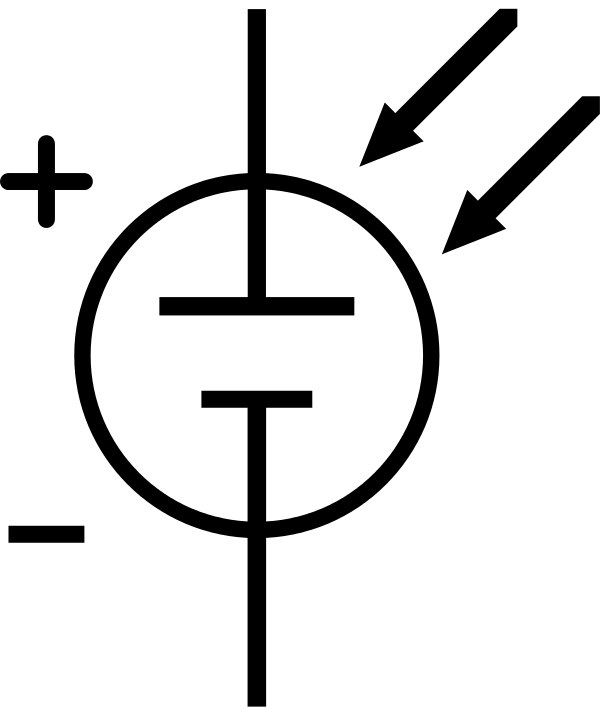
\includegraphics[width=0.2\textwidth]{img/Photovoltaic_cell.png}
	\caption{Symbol of a PV cell.}
	\vspace{-10pt}
\end{wrapfigure}

When a photon hits a piece of silicon, one of three things can happen:  
\begin{itemize}
	\item The photon can pass straight through the silicon (this generally happens for lower energy photons) 
	\item The photon can reflect off the surface 
	\item The photon can be absorbed 
\end{itemize}

When a photon is absorbed in the semiconductor, it creates mobile electron-hole pairs. If a load is placed across the cell as a whole, these highly excited, non-thermal electrons will flow out of the p-type side into the n-type side, lose energy while moving through the external circuit, and then flow back into the p-type material where they can once again re-combine with the valence-band holes they left behind. This generates an electromotive force, and thus some of the light energy is converted into electric energy.

\subsection {Circuital Model}

\begin{wrapfigure}{r}{0.4\textwidth}
	\centering
	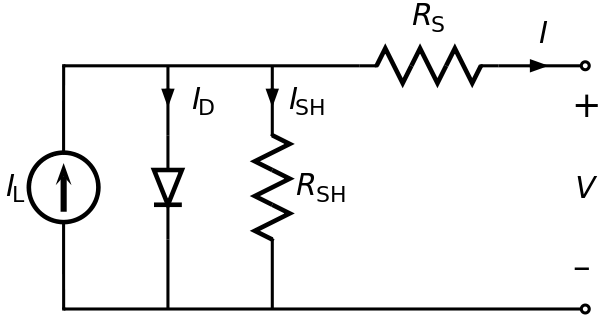
\includegraphics[width=0.4\textwidth]{img/601px-Solar_cell_equivalent_circuit.png}
	\caption{Solar cell equivalnet circuit}
	\vspace{10pt}
\end{wrapfigure}

An ideal solar cell may be modeled by a current source in parallel with a diode but in practice no solar cell is ideal, so a shunt resistance and a series resistance component are added. \footnote{A shunt is a device which allows  electric current  to pass around another point in the  circuit  by creating a low resistance path.} The values of $I_{0}$, $R_{S}$, and $R_{SH}$ are dependent upon the physical size of the solar cell. In comparing otherwise identical cells, a cell with twice the surface area of another will have double the $I_{0}$ and half the $R_{S}$ and RSH. Indeed it has twice the junction area across which current can leak.



\subsection{Parameters}

The short-circuit current and the open-circuit voltage are the maximum current and voltage from a solar cell. However, at both of these operating points, the power from the solar cell is zero. The "fill factor"(FF), is a parameter which determines the maximum power from a solar cell. It is defined as : 

\begin{align}
FF &= \frac{MaximunPower}{V_{oc}I_{sc}}  = \frac{I_{mp}V_{mp}}{V_{oc}I_{sc}} \\
\intertext{Where:}
V_{oc} &= \text{Open Circuit Voltage} \\
I_{sc} &= \text{Short Circuit Current} 
\end{align}

\begin{wrapfigure}{r}{0.5\textwidth}
	\centering
	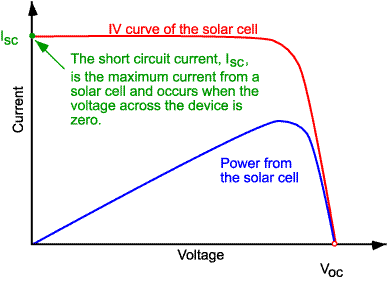
\includegraphics[width=0.5\textwidth]{img/IV-ISC.png}
	\caption{IV curve.}
\end{wrapfigure}


%
%\begin{wrapfigure}{r}{0.6\textwidth}
%	\centering
%	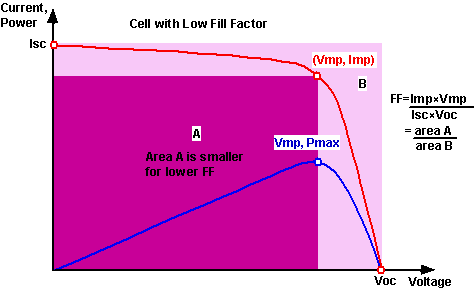
\includegraphics[width=0.6\textwidth]{img/FFL.png}
%	\caption{FF graph.}
%\end{wrapfigure}


Graphically it is the area of the largest rectangle which will fit in the I-V curve. In the cell, the higher the voltage the higher the possible FF. However, large variations in open-circuit voltage within a given material system are uncommon. For example, at one sun $(1000 W/m^2)$ the difference between the maximum open-circuit voltage measured for a silicon laboratory device and a typical commercial solar cell is about 120 mV. Their maximum fill factors are respectively of 0.85 and 0.83. However, the variation in maximum FF can be significant for solar cells made from different materials. For example, a GaAs (Gallium Arsenide) solar cell can have a FF of about 0.89. 

The most commonly used parameter to compare the performance of solar cells is efficiency which is defined as the ratio of energy output from the solar cell to input energy from the sun. 

\begin{align}
 \eta &=\frac{FF*V_{oc} * I_{sc}}{P_{in}}  
 \intertext{Where:}
 P_{in} &=  \text{Solar Input Energy}
\end{align}
In addition to the performance of the solar cell itself, the efficiency depends on the spectrum and intensity of the incident sunlight and on the temperature of the solar cell. Indeed $V_{OC}$ is reduced linearly with increasing temperature. The magnitude of this reduction is inversely proportional to $V_{OC}$, hence cells with higher values of $V_{OC}$ suffer smaller reductions in voltage with increasing temperature.  

As regards to the spectrum, a photon need only have greater energy than the band gap in order to excite an electron. Much of the solar radiation reaching the Earth is composed of photons (blue and violet end of the spectrum) with energies greater than the band gap of silicon. These higher energy photons will be absorbed by the solar cell, but the difference in energy between these photons and the silicon band gap is converted into heat (via lattice vibrations \textendash ~called phonons) rather than into usable electrical energy.  

Moreover, in order to have a reasonable chance of capturing a photon, the n-type layer has to be thick. This increases the chance that an ejected electron will meet up with a hole in the material before reaching the p-n junction. 

These effects produce an upper limit on the efficiency of silicon solar cells. The use of multiple semiconducting materials allows the absorbance of a larger range of wavelengths, improving the efficiency.  

\section{Multijunction Cells}

Multijunction photovoltaic cells are composed of more than one single pn-junction and usually they are between two and four. Spatially, these pn-junctions are stacked one on top of each other in order to capture as much as possible of the light frequencies. However, this disposition leads to several problems. The two biggest constraints to the design of a multijunction cell are how to let the light penetrate down to the very last junction and how to handle the current generated by the different junctions.

\subsection{Light Penetration}

In order to obtain the highest efficiency out of a multijunction cell and to provide energy, it is necessary to have every single junction irradiated by enough light. 
However, if we stack different cells on top of each other, our intuition would suggest that only the first cell is going to be irradiated, while the next cell will be on the shadow of the top one.  
What actually happens is that light of specific wavelength does not interact with materials that are not multiples of that wavelength, this property is exploited to let light penetrate the first layer of a multijunction cell down to the further ones.  Exploiting this property, to absorb the light in the most efficient way means to choose which wavelength absorb first, hence if we absorb first the light of wavelength $2n$ the junction interacting with wavelength $n$ won't be able to absorb anything. The junctions that absorb the smaller wavelength are so stacked on top of the junctions with bigger wavelength.  

\subsection{Current Flow}

Different pn-junction provides different current, however, as any electrical component, even they need to obey the Kirchhoff law of current. This means that the current which flows into a pn-junction must be equal to the current that flows out of it.  In order to manage the different currents produced by the different junctions two main designs emerge: the monolithic multijunction and the stacked multijunction. 

\subsection{Monolithic Structure}

In a monolithic multijunction the different layers are stacked directly one on top of the other and the current flows between the different cells in series. If a junction produces the wrong current it will act as load, heating the device itself, heading to a loose of efficiency, and consuming power directly.  For this reason the single junctions must be carefully tuned to produce the right amount of current, this is achieved modifying slightly the dope amount.  

\subsection{Stacked Structure}

Opposed to the monolithic cell, the stacked cell are composed of several different layers, but each layer is completely isolated from the others.  This design avoids completely the issues about the possible differences in current production for each cell. However, as trade off, the stacked cells require transparent contacts that are still not sufficiently developed.  Because of that, the most widely developed and used are the monolithic one, so the rest of the article will explore the implementation of such multijunction cells.

\section{Technical exploration of the multijunction cell}

After a lot of iterations in their design, the modern multijunction cell is composed of different, but extremely similar, layers connected by a tunnel junction. Every single layer of the monolithic solar cell consists of:

\begin{enumerate}
	\item Windows 
	\item Emitter 
	\item Base 
	\item Back Surface Field (BSF) 
\end{enumerate}
The layers are different because of the different combinations of materials used for the components, each of which is the most appropriate to absorb a particular wavelength. Of course every single component must be transparent to the light that needs to hit the underlying cells. 

\subsection{Components}  

Like every single junction photovoltaic cell, the light is converted into energy thanks to the depletion region between the base and the emitter.  

\subsubsection{Windows and Back Surface Field}  
In order to avoid losses by recombination of electrons, a window and a back surface field are used.  The window, which is on top of the layer, is used to reduce the surface recombination velocity while the BSF, which is on the bottom of the layer, is used to reduce the scattering of carriers towards the tunnel junction.  

\subsubsection{Tunnel Junction}

A tunnel junction is a fundamental piece of every multijunction cell, it is a very high doped pn-junction which serves two main purposes: junctions isolation and low electrical resistance between the different layers.  

The presence of a tunnel junction isolates the p-region from the top cell from the n-region of the lower cell.  Without such isolation we would have an inverse junction between the different layers and the photo-voltage would drop significantly.  

Because of the high level of doping of the tunnel junction the bandgap between the two regions of the tunnel junction is extremely low, this cause the tunnel effect which lets the electrons pass practically undisturbed between the different layers.  Using the tunnel effect we achieve a contact between the different layers without any practical power loss.


\section{Material}

Multi-junction cells use a combination of materials from the 3rd  and 5th column of the periodic table and because of this, these cells are usually called III-V multijunction cells.

Some applications with GaAsSb heterojunction give the opportunity to change the doping level of the material: it is in fact possible to obtain the same current with a lower doping. A tunnel diode based on a GaAsSb heterojunction, has a tunneling distance lower than other compounds. On the other hand its valence band is higher than the valence band of the adjoining p-doped layer. This reduces the tunneling distance and its current. In fact the current depends exponentially on the tunneling distance. Hence the voltage becomes much lower than the one in tunnel junction of other materials.  

\subsection{Three-Junction cell}

\begin{wrapfigure}{r}{0.3\textwidth}
	\centering
	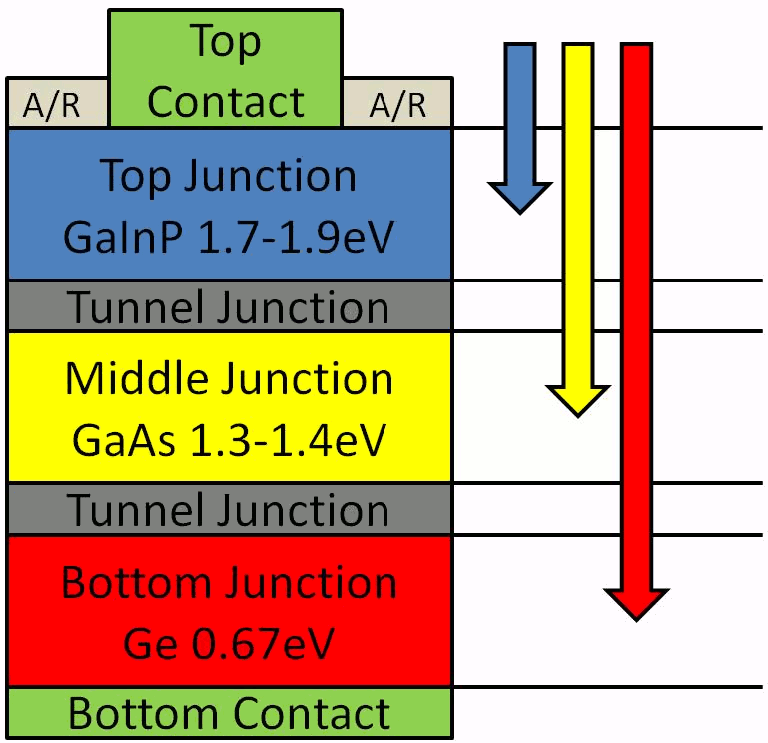
\includegraphics[width=0.3\textwidth]{img/f2big.png}
	\caption{Structure of a three junction phovoltaic cell.}
\end{wrapfigure}

Between the multi-junction cells the most common structure has three layers.  

\begin{wrapfigure}{l}{0.55\textwidth}
	\centering
	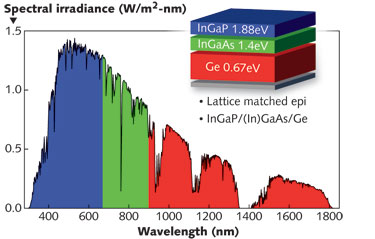
\includegraphics[width=0.45\textwidth]{img/1212LFW04f2.jpg}
	%\vspace{-50pt}
\end{wrapfigure}

To choose the best combination of semiconductor materials for a triple junction, we look at the frequency specifications. Specifications which led to use Indium Gallium Phosphide (InGaP) for the top layer, Gallium Arsenide for the middle layer, and Germanium for the bottom one. This InGaP/GaAs/Ge model is one of the best for triple-junction cell in terms of efficiency which, in concentrated sunlight, reaches values around 40\%. These materials in fact make the cell work with a larger range of photons, furthermore the thermalization loss is critically minimized. This structure presents a band gap for the top junction of 1.88eV, a middle junction gap around 1.4eV and a lower junction gap of 0.66eV. The top layer absorbs wavelengths from 300 nm to 670 nm, the middle layer consequently receives until 900 nm wavelength light while the Germanium layer works between 900 nm and 1800 nm. 

Among the several structures used it is also possible to find materials such as Indium Gallium Nitride (InGaN) or Indium Phosphide (InP). The choice of these materials is preferable if specific band gaps are required. For the InGaN, it is possible to tune the band gap from 0.8eV to 3.5eV while for InP structures the gap can reach 1.35eV. Both these materials don't seem to be competitive in terms of cost effectiveness and for now just remain ideal materials.

\subsection{Other Multijunction cell structure}

Beside the three-junction cells there are designs using more then three junctions.  

A four-junction model can be GaInP/AlGaAs/GaAs/Ge with band gap energies of 1.90/1.43/1.04/0.67 eV. The current in a four-junction is 33\% smaller than the one in a three-junction while its maximum theoretical efficiency limit in concentrated light is around 58\%, its realistic value is around 45\%.  

Two possible five-junction configurations are AlGaInP/GaInP/AlGaInAs/GaInAs/Ge or AlGaInP/AlGaInAs/GaInAs/GaInNAs/Ge. This last structure has a realistic efficiency  of 55\% thus it's regarded as an advanced five-junction structure. 

Six-junction cells have the following material structure: GaInP/GaInP/AlGaInAs/ GaInAs/GaInNAs/Ge. The potential efficiency of this structure could be around 58\% and under specific conditions this structure is capable of producing 5.25 V at 1 sun and over 6 V at 500 suns.

\section{Efficiency}
As previously explained there are several limitations in a solar cell. They determine a maximum theoretical efficiency, for single-junction solar cells with no light concentration, of 33\% but of course because of practical issues the theoretical values will never be reached. However, semiconductors like silicon and GaAs are close to this optimal bandgap and record efficiency values of 25.6 percent and 28.8 percent have already been reached in laboratory. Another fact is to be considered: from the laboratory the studies must be brought to an industrial application and here, inevitable losses in the module cause a further reduction leading to an industrial module limit of 25 percent. It can be assumed that such high-end modules will be available in 2050. Yet it’s always to be remembered that cost competiveness is not only related to high efficiency so it’s not possible to foresee now it’s developments. 

\begin{figure}[h]
	\centering
	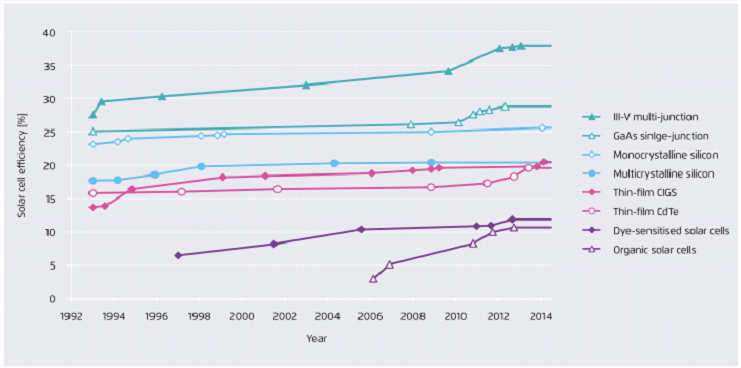
\includegraphics[width=0.8\textwidth]{img/Immagine.png}
	\caption{In this figure we can see the development of the various types of solar cells since 1992}
\end{figure}

Multijunction devices allow to bypass some of single-junction cells limitations. By using more junctions, it's possible to make sure that each subcell converts a specific part of the sun´s spectrum, permitting to reach theoretical efficiency limits of 46 percent for dual-junction and 52 percent for triple-junction solar without concentration. Theoretically, an infinite number of junctions would have a limiting efficiency of 86.8\% under highly concentrated sunlight.

Due to the fact that they are mainly used with concentrator devices, the concentration ratio of the incident light needs to be considered because the voltage of a solar cell increases logarithmically with the  concentration. Thus efficiency  under  concentrated  light is  always  higher  than  at one-sun. In this table we can see top efficiencies  recorded using different combinations of materials and at different light concentration levels.

\section{Market and distribution of the MJ}

The cost competiveness of an energy producing technology is often rated by the levelized cost of energy ( LCOE )  which is  the  total  cost  of  the  system  divided  by  its  lifetime  energy production. This means that high PV efficiencies  are  essential  for lowering  the  LCOE  as  more  energy can  be produced from the same installation area. However if by increasing system costs the  benefit  of  higher  energy  production is outweighed, no benefits is achieved.   

III-V multi-junction solar  cells  are essentially more expensive than conventional Silicon-based solar cell technologies on the same cell area. In fact, the price of typical GaAs or Ge wafers is more or less a hundred times the one for a Silicon wafer. This means that even if their efficiency is about twice as high, III-V multi-junction solar cells are currently too expensive to be used in flat-plate modules on Earth.   However, large-area III-V multi-junction solar cells are nowadays standard in space applications as the major cost measure are €/kg rather than €/Wp. This is due to the high launch costs and the importance of spacecraft attitude control. Besides cost aspects III-V multi-junction solar cells  are  also  particularly  suitable  for  the  need  in  space  due  to  their  radiation  hardness,  small temperature coefficients, high reliability and the combination of high voltage and low current. In fact the development and continuous improvement of III-V multi-junction solar cells has been driven by the relatively stable space market for a long time.  





 In recent years they are not  only used in space applications but they entered also the terrestrial PV market, in  concentrating  photovoltaic  (CPV)  systems which use  concentrating  optics  to  reduce  the  expensive  cell  area,  which  allows  competitive  LCOE.  Lately, many  companies  have  implemented  this  idea  with  a  variety  of  CPV  concepts  and  an  increasing number of installations worldwide.   

 \begin{wrapfigure}{r}{0.4\textwidth}
	\centering
	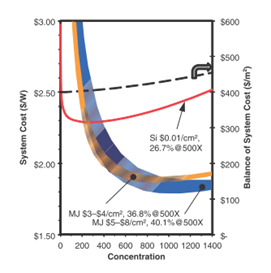
\includegraphics[width=0.4\textwidth]{img/sadasd.png}
	\caption{Comparison of the cost of different system.\label{fig:aa}}
\end{wrapfigure}
Refering to the figure~\ref{fig:aa} it’s possible to make an hypothetical comparison between the costs of a CPV plant and the ones for a normal PV plant. If the complete plant costs are known, it’s quite easy to calculate the impact of different cell prices and efficiency combinations on the overall project. From the figure (which doesn’t use real but hypothetical data) it’s clear that the higher efficiency MJ cells will always result in a lower system cost (€/W) at sufficiently high concentration. This also means that the roadmap to higher efficiency will most likely drive CPV systems to keep increasing concentration.   

Still, this kind of technology is expensive and that’s why also other approaches are being studied. For example another  approach, which  could  reduce  the cost  of  III-V  solar  cells,  is  to re-use  the  expensive semiconductor substrate. The resulting thin-film solar cells have high efficiencies and can be used in flexible modules. This approach is  seen  as  a  way  to  enable  the  use  of  III-V  solar  cells  in  flat-plate modules in building-integrated as well as rooftop applications in the near future. By the way III-V solar cells are also used in several niche applications such as laser power converters and thermophotovoltaics (TPV).
 

\section{Conclusion}

The field of the photovoltaic research is moving extremely fast toward more efficient solar cell. As stated in this paper multijunction solar cells are, by now, the most efficient but, since they are still complex to produce in industrial quantity, they won't land in the consumer market very soon.

Major advancements are still possible, both in the design of the multijunction cell and in the production methodology. In fact research is developing both ways and the result are showing to be promising.

\begin{thebibliography}{9}
\bibitem{}
\url{http://www.sciencedirect.com/science/article/pii/S2215098615000245}
\bibitem{}
\url{http://science.nasa.gov/science-news/science-at-nasa/2002/solarcells/}
\bibitem{}
\url{http://pvcdrom.pveducation.org/DESIGN/SURF_MIN.HTM}
\bibitem{}
\url{http://academic.evergreen.edu/curricular/matterandmotion/chem_phys/solar_cells.pdf}
\bibitem{}
	"III–V multijunction solar cells for concentrating photovoltaics", by Hector Cotal, Chris Fetzer, Joseph Boisvert, Geoffrey Kinsey, Richard King, Peter Hebert, Hojun Yoon and Nasser Karam, Spectrolab \url{http://www.spectrolab.com/pv/support/Cotal_III_V_multijunction_photovoltaics.pdf}
\bibitem{}
	"Concentrated Solar Photovoltaics" by Jeffrey Weisse \url{http://large.stanford.edu/courses/2010/ph240/weisse2}
\bibitem{}
	"Solar cell generations over 40\% efficiency" R.R. King (2012) 
\bibitem{}
	\url{http://www.ise.fraunhofer.de/en}
\bibitem{}
	Multi-junction III–V solar cells: current status and future potential. Authors: Masafumi Yamaguchi , Tatsuya Takamoto, Kenji Araki, Nicholas Ekins-Daukes 
\bibitem{}
	Emerging and Novel Photovoltaic Technologies. Author: The Applied Research Institute for Prospective Technologies  
\bibitem{}
	Design of III-V multijunction solar cells on silicon substrate. Author: Nikhil Jain 

\end{thebibliography}

\end{document}
